%%%%%%%%%%%%%%%%%%%%%%%%%%%%%%%%%%%%%%%%%%
\section{Experimental Study}\label{sec:experiments}
%%%%%%%%%%%%%%%%%%%%%%%%%%%%%%%%%%%%%%%%%%
% Phase 8 rewrite (drafting steps 3-4). Every empirical number is bound to a
% validated artifact of evidence release rel-2026-07-20-67d9345f9 via a
% "% BIND:" comment. No ablation or component-contribution content appears in
% this section (DEFERRED_TO_PHASE_12_SUPPLEMENT_ONLY).

On CEC2017 \dtgsk{} attains the best overall Friedman
mean rank in the seven-algorithm panel, placing first at three of four
dimensions and second at $D = 30$; on CEC2011 it is likewise second, with
a Holm-significant loss to \egsk{}. The CEC2020 and CEC2013LSGO legs,
added under a registered analysis-plan addendum, are reported in
Sections~\ref{sec:exp:cec2020} and~\ref{sec:exp:cec2013lsgo} at their
registered evidential tiers, and the five-suite synthesis is confined to
Section~\ref{sec:exp:discussion}. The evidence below is reported at that
resolution --- tier by tier, with the unfavorable cells stated alongside
the favorable ones --- because the dimension-resolved pattern, not a single
aggregate, is what the dimension-tiered design predicts and what the data
support. Every comparative statement is scoped to this panel; no
field-wide claim is made.

%------------------------------------------------------------------
\subsection{Experimental Setup}\label{sec:exp:settings}
%------------------------------------------------------------------

\paragraph{Evidence discipline.}
Every empirical value in this paper derives from a versioned, immutable
evidence release: all seven
panel algorithms were re-run in-repository under one identical
protocol, and the analysis pipeline
(SciPy~1.15.3) runs
restricted so that it can read only the three such releases identified in
the Data Availability Statement --- the primary three-suite release and
the two later, separate, non-superseding single-suite releases for
CEC2013LSGO and CEC2020 --- never staging data and never
literature-copied numbers
presented as comparable.
% BIND: environment_record.json (release_id, strict_source, packages); evidence_release_manifest_cec2013lsgo.json; evidence_release_manifest_cec2020.json
One provenance qualification applies: the \egsk{} panel cells derive
from the committed reference results of the runnable \egsk{} port,
whose late local polish uses SciPy-SLSQP, whereas the original
algorithm's late refinement is a sequential-quadratic-programming
polish~\cite{jawad2024egsk}, realized as MATLAB fmincon in the family's
reference implementation. The substituted routine is a search
component rather than a cosmetic finishing step: it consumes part of the
same evaluation budget and can move the returned solution, so the \egsk{}
cells reported here are properties of this port and not of the published
implementation. Cross-implementation runtime and environment comparability
is therefore limited, no runtime-superiority claim is made anywhere in this
paper, and no claim of numerical equivalence to the published \egsk{} is
made in either direction.
% BIND: LM-04 (papers/governance/data_ledger.csv; comparability_audit.md)

\paragraph{Suites, budgets, and metrics.}
Table~\ref{tab:protocol} summarizes the frozen protocol. The primary
suite is the CEC2017 bound-constrained suite~\cite{awad2016problem}:
29 functions (F1, F3--F30) at $D \in \{10, 30, 50, 100\}$, 51 runs per
(function, dimension), $\mathrm{MaxFES} = 10^{4} \cdot D$, and final
error $f(\mathbf{x}) - f(\mathbf{x}^{*})$ with errors below $10^{-8}$
treated as zero per the suite's reporting convention. F2 is excluded under the
adopted CEC2017 protocol because of documented instability and
difficult-to-reproduce behavior, uniformly in every panel cell.
% BIND: PR-01, PR-04, PR-05 (claims matrix; benchmark_protocol_audit.md)
The real-world suite is CEC2011~\cite{das2011cec2011}, which supplies
real-world problem \emph{formulations} executed as a standardized benchmark:
22 problems at their native dimensions, 25 runs per problem,
$\mathrm{MaxFES} = 150{,}000$. This is breadth of application formulation,
not evidence of deployment performance. The endpoint is the raw best objective
value, and negative optima occur on some problems. The error column
is NaN by design on problems without published optima, where
best-fitness is authoritative.
Infeasible evaluations --- for instance a failed trajectory integration
or an out-of-domain intermediate value on the orbital-mechanics problems
--- receive the reference implementation's standard infeasibility penalty ($10^{30}$),
applied identically for all seven algorithms, so a feasible candidate is
always preferred to an infeasible one at selection.
% BIND: PR-02, PR-04 (claims matrix; data_ledger.csv); benchmarks/cec_suite_python/cec2011/_constants.py (NAN_PENALTY)
Finally, CEC2013~\cite{liang2013cec2013} is reported as a second
comparison suite for breadth of comparison under the same protocol:
28 functions at $D \in \{10, 30, 50\}$, 51 runs,
$\mathrm{MaxFES} = 10^{4} \cdot D$, same error convention.
% BIND: PR-03 (claims matrix); captions_registry conventions
Two further suites were added after the primary release under a
registered analysis-plan addendum, with their protocol facts fixed at
registration. The CEC2020 bound-constrained suite~\cite{yue2020cec2020}
is the pre-registered \emph{confirmatory} suite: 10 functions at
$D \in \{5, 10, 15, 20\}$, with F6 and F7 undefined at $D = 5$, giving
38 protocol cells; 30 runs per cell; a dimension-dependent budget of
$\mathrm{MaxFES} = 5 \times 10^{4}$, $10^{6}$, $3 \times 10^{6}$, and
$10^{7}$ at $D = 5/10/15/20$; and the same error basis and $10^{-8}$
floor as CEC2017.
% BIND: SAP addendum Section 2 (protocol facts registered before any CEC2020 datum); RS-12
The CEC2013LSGO large-scale suite~\cite{li2013lsgo} --- distinct from
the bound-constrained CEC2013 suite above --- is the post-hoc,
\emph{family-internal} suite: 15 functions at their native $D = 1000$
(F13 and F14 at 905 through their overlap), 25 runs,
$\mathrm{MaxFES} = 3 \times 10^{6}$, and the raw best-objective basis
(the error column is not populated on this suite). Its F3, F6 and F10
were executed with the transformed Ackley variant, so results on those
three functions are not comparable to published values obtained on the
raw variant, and no such comparison is drawn anywhere in this paper.
% BIND: SAP addendum Section 2; RS-13; production_deviation_record.md D-8.2 (Ackley variant)

\begin{table}[H]
\caption{Frozen evaluation protocol, one row per suite. The seed schedule is
optimizer-independent
and keyed by (dimension, function, run); the full-schedule
recomputation audit for the primary release (70{,}813 rows, 0 mismatches) is
part of the
released evaluation record, and the CEC2020 and CEC2013LSGO banks were
audited for cross-algorithm seed identity at promotion (0 mismatches).
CEC2020 scores 38 protocol cells (F6 and F7 are undefined at $D = 5$);
CEC2013LSGO runs F13 and F14 at their native $D = 905$.}\label{tab:protocol}
\centering
\tablesize{\scriptsize}
\setlength{\tabcolsep}{4pt}%
\begin{tabular}{lccccc}
\toprule
\textbf{Suite} & \textbf{Problems} & \textbf{Dimensions} & \textbf{Runs} & \textbf{MaxFES} & \textbf{Endpoint} \\
\midrule
CEC2017 (primary) & 29 (F1, F3--F30) & 10/30/50/100 & 51 & $10^{4}\cdot D$ & error ($<10^{-8}\!\to\!0$) \\
CEC2011 (real-world) & 22 & native & 25 & $150{,}000$ & raw best objective \\
CEC2013 (second comparison) & 28 (F1--F28) & 10/30/50 & 51 & $10^{4}\cdot D$ & error ($<10^{-8}\!\to\!0$) \\
% F6/F7-at-D5 exclusion stated in the caption; repeating it in the cell
% overfilled the line by 45pt (build-hygiene gate).
CEC2020 (confirmatory) & 10 & 5/10/15/20 & 30 & $5{\cdot}10^{4}/10^{6}/3{\cdot}10^{6}/10^{7}$ & error ($<10^{-8}\!\to\!0$) \\
CEC2013LSGO (family-internal) & 15 & 1000 (F13/F14: 905) & 25 & $3\times10^{6}$ & raw best objective \\
\midrule
Seed schedule & \multicolumn{5}{c}{$s(D,f,r) = (20240620 + 1000003\,D + 1000033\,f + 1000037\,r) \bmod (2^{31}{-}2) + 1$} \\
Generator & \multicolumn{5}{c}{counter-based Threefry; identical schedule for all seven optimizers on every suite} \\
Initialization & \multicolumn{5}{c}{runner-generated shared $X_{0}$; exception: \dtgsk{} self-init from the same stream} \\
Significance & \multicolumn{5}{c}{$\alpha = 0.05$; Holm at $m{=}6$ per dimension (across-function layer); tie band $|\Delta| < 10^{-8}$} \\
\bottomrule
\end{tabular}
% BIND: papers/governance/seed_and_pairing_audit.md (formula, base seed, audit counts); PR-04; PR-06; SAP addendum Sections 2 and 12 (CEC2020/CEC2013LSGO protocol facts, unified seed policy, pairing audits)
\end{table}

\paragraph{Panel, pairing, and seed-paired start.}
The comparison panel is exactly the seven-algorithm GSK family of
Table~\ref{tab:panel}; comparator configurations follow the family's
shipped reference implementations
(Table~\ref{tab:comparator-params-main};
Section~\ref{sec:alg:overview} discloses where these differ from the
source papers), and \dtgsk{} runs the single hash-frozen configuration
(Table~\ref{tab:parameters}), identical across the four bound-constrained
suites with no per-suite tuning. On CEC2013LSGO alone it adds two
linkage-block-size entries, for $D = 905$ and $D = 1000$, set to the
benchmark's own declared group size of 50 rather than fitted to any
observed result; without them the shipped table falls back to a block
size of 10. The values were added while LSGO results already existed, so
outcome-blindness is not asserted for them; the rule, the rationale, and
the timing are disclosed in Supplementary Section~S7.
% BIND: production_deviation_record.md D-8.4 (linkage_block_size_by_dim 905/1000 -> 50); RS-13
That configuration was, however,
selected on CEC2017, which is therefore the \emph{development} suite and is
selection-exposed; CEC2011 and CEC2013 were not consulted during
configuration selection and serve as \emph{corroborative} suites, not
independent development benchmarks; CEC2020 is the \emph{pre-registered
confirmatory} suite, whose analysis plan, hypotheses and outcome wording
were committed before any CEC2020 result existed; and CEC2013LSGO is
\emph{post-hoc exploratory} and family-internal, its descriptive layer
having been inspected before registration. The CEC2017 standing should
accordingly be
read as development-suite performance, the CEC2011/CEC2013 standings as
corroboration, the CEC2020 standing as the registered confirmatory test,
and the CEC2013LSGO standing as exploratory. Six full-panel candidate
configurations, including the one
selected, were compared against the seven-algorithm panel on CEC2017 before
promotion; the full development protocol and the scope of that count are
disclosed in the Supplementary Materials, Section~S5.
% BIND: captions_registry (ART-PARAMS caption: no per-suite tuning, bound-constrained scope); CN-02; SAP addendum Section 1 (suite roles); RS-12; RS-13
Runs are paired across optimizers by common seed, problem instance, and
run index: within each suite all seven optimizers use the identical seed
schedule of Table~\ref{tab:protocol} on byte-identical problem instances.
% BIND: papers/governance/seed_and_pairing_audit.md Sec.4
For the six comparators, run $r$ additionally starts from the same
runner-generated initial population $X_{0}$; \dtgsk{} is the one
documented exception --- it self-initializes its own $5 \cdot D$ population
from the same seed-paired random stream, so its initial population is drawn
under the identical seed but is \emph{not} byte-identical to the shared
$X_{0}$. Pairing is therefore by common seed/problem/run rather than by an
identical starting population for \dtgsk{}; the exception is recorded in
the protocol exhibit and the pairing audit rather than hidden.
% BIND: PR-06 (claims matrix); seed_and_pairing_audit.md
One evidence gap is disclosed up front. At the time of the frozen analysis,
APGSK per-run records on CEC2017 were available only at $D = 100$, the
result of a sidecar-overwrite anomaly in the evidence tree. Seeds and
summary values for $D \in \{10, 30, 50\}$ were verified equivalent from the
generation logs, so run-level statistics against APGSK at those dimensions
were treated as disclosed-unavailable and were never imputed. The primary
across-function test on per-function means --- the same test used for every
comparator --- still applies to APGSK. Those run-level records were
subsequently recovered and are present in the released bundle; only the
non-deterministic wall-clock runtime remains unavailable at those
dimensions. The recovery was deterministic, from the seed-identical per-run logs, and reproduces the frozen APGSK summaries exactly; because the primary analysis was already frozen when it landed, the manuscript conservatively retains the function-level basis reported here, and no headline number is affected.
% BIND: negative_findings.md item 8; captions_registry [APGSK-GAP]

% Phase 8 assembly: the T-PANEL roster float (label tab:panel) is typeset once,
% at its outline-bound position in Section 3.7 (outline.md X5); the reference
% above resolves there. A duplicate float previously defined here was removed
% to fix the multiply-defined label (build_record.md, Phase 8).

\paragraph{Environment and determinism.}
All runs were executed on a 22-logical-core Windows workstation
(Windows 11, build 10.0.26200) under Python~3.10.11 with Numba~0.64.0
JIT kernels. Campaigns parallelize only across independent
(function, dimension, run) cells --- 15 worker processes, with no parallelism
inside a run. Every cell records an environment.json
manifest including the git commit, JIT state, and floating-point
probe hashes of the shared RNG, the \dtgsk{} kernels, and the suite
evaluators. The comparator-specific update kernels are \emph{not} covered
by a numerical probe: their JIT state is recorded, but their numerical
identity across producer commits rests on the shared-kernel probes and code
history rather than on a direct hash.
% BIND: fp_environment_audit.md Sec.2 (residual limitation); N-017
% BIND: benchmarks/cec_reference_results/cec2017/dt-gsk/environment.json (cpu 22, platform, python, numba, workers, fp_regime); fp_environment_audit.md Sec.2 (comparator-kernel probe gap)
The analysis bundle records its own environment (NumPy~2.2.6,
SciPy~1.15.3, pandas~2.3.3).
% BIND: environment_record.json (packages)
For \dtgsk{}, every objective evaluation, including polish and escape
evaluations, is charged through the strict budget-accounting path
described in Section~\ref{sec:algorithm}; the reference-faithful
comparator ports instead retain their original budget-crossing
semantics, evaluating the terminal batch in full and counting only its
in-budget prefix. No optimizer is therefore charged more than
$\mathrm{MaxFES}$; AGSK and APGSK additionally stop on reaching the
$10^{-8}$ target error, which ends $1{,}845$ of the primary evidence
release's $75{,}250$ runs
(AGSK $962$ and APGSK $883$, summed over CEC2017 and CEC2013; by suite,
$742$ and $1{,}103$ respectively) below the cap, while
the remaining five optimizers implement no such criterion and always consume
the full budget. That crossing falls only on the terminal
generation, so the uncounted rows enter no incumbent and no later state.
A controlled cell was constructed so that the budget is not a multiple of the
population, forcing the crossing for every optimizer that exhibits it.
Overwriting all such rows leaves the returned solution, its fitness and the
charged budget bit-identical for all seven. The inertness itself follows
structurally, from the prefix-only incumbent scan and immediate loop exit, so
the crossing confers no search advantage.
% Evidence: tests/regression/test_budget_crossing_semantics.py -- with MaxFES
% deliberately non-divisible by NP, the six ports leave 8-50 uncounted terminal
% rows (dt-gsk 0); poisoning every one of them with 1e300 leaves best_fitness,
% nfes and best_x bit-identical. See benchmark_protocol_audit_part2.md Sec.7.5.
Runs are budget-exact and
repeat-identical; byte-identical reproduction at $D \geq 50$ requires
single-threaded numerical kernels (a fixed reduction order), and the
shipped runs use one compute thread per run, so the repeat-identical
property holds for them but is not guaranteed under a different thread
configuration. This determinism is established for \dtgsk{} in its
declared single-threaded environment; it is not claimed for the
comparator ports across producer commits, where a re-execution of the
six comparators was verified \emph{not} to reproduce the frozen
scientific columns exactly (a floating-point path shifted between the
producing commits, amplified on a minority of runs by the chaotic
search). The released evidence is unaffected --- it is the archived
output of the original campaign --- but a bit-identical re-timing of the
comparators under current code is not achievable, which is why the
runtime table is reported for \dtgsk{} only. Per-run raw
CSVs, seed schedules, and verification manifests ship with the
release (see the Data Availability statement).
% BIND: MT-11, CN-02 (claims matrix); implementation_correspondence.md note 2 (single-thread byte-stability precondition)
% BIND: benchmark_protocol_audit_part2.md Sec.7.5 (boundary semantics: DT-GSK strict truncation vs comparator terminal-batch overrun; counted budgets exactly MaxFES for all seven)
No generative-AI system designed or executed any experiment, and none
produced or computed any reported number; two large language models were
used for language editing, the drafting of descriptive prose, structural
and consistency review, and software-engineering support, as
declared in full in the back matter (Use of Generative Artificial
Intelligence).
% BIND: phase_08/build_record.md note AG-0007 (GenAI methods-level disclosure; back-matter placement)

\paragraph{Statistical protocol.}
Hypotheses are stated once here. For each comparator and dimension,
a two-sided Wilcoxon signed-rank test~\cite{wilcoxon1945individual}
is applied to the 29 paired per-function mean errors
($H_{0}$: the paired differences are symmetric about zero), with
Holm step-down correction~\cite{holm1979simple} across the
six simultaneous comparators at that dimension ($\alpha = 0.05$).
Win/tie/loss counts use the tie rule $|\Delta| < 10^{-8}$ --- the same
$10^{-8}$ the suite uses to floor errors to zero, here applied to the
per-function mean difference. This single absolute band is a coarse
convention across functions of very different scales, so the win/tie/loss
tallies are a \emph{descriptive} companion only. The Friedman test ranks
\emph{within} each function and is therefore invariant to per-function scale;
the Wilcoxon signed-rank test, applied here across per-function mean
differences, ranks the absolute differences \emph{across} functions and is
accordingly \emph{not} scale-invariant --- functions with larger numerical
ranges carry more weight in it. The tie band itself affects no significance
decision, but this cross-function scale heterogeneity is a genuine limitation
of the paired test, and is one reason the Friedman ranking is treated as the
primary aggregate. Every
test is accompanied by its \emph{aligned} effect size: because the
across-function test is a matched-pairs Wilcoxon, the tabulated effect size is
the matched-pairs rank-biserial correlation
$r = (R^{+} - R^{-})/(R^{+} + R^{-})$, where $R^{+}$ is the rank sum of the
comparisons favoring \dtgsk{}, so that $r > 0$ favors \dtgsk{}. (The released
workbook stores the same quantity under the mirrored column names
w\_plus/w\_minus, whose roles are exchanged relative to
$R^{+}/R^{-}$. Its rank\_biserial column already carries the sign
convention used here.) The
unpaired Vargha--Delaney $A_{12}$~\cite{vargha2000critique} ($A_{12} > 0.5$
favors \dtgsk{}; the conventional 0.56/0.64/0.71 guidelines label magnitudes)
is retained as a descriptive companion in the released workbooks. Zero differences under the tie rule
($|\Delta| < 10^{-8}$) are discarded before ranking
(zero\_method=`wilcox'), and the reported $p$-values are produced by
this repository's own pure-\textsc{NumPy} wilcoxon\_paired routine
using the normal approximation with continuity correction. That routine is
cross-checked against scipy.stats.wilcoxon
(zero\_method=`wilcox', correction=True,
method=`approx') in the released cross\_check.json; of the
three audited cells, the two with a defined statistic agree on it to a
relative tolerance of $10^{-12}$ and on the $\alpha = 0.05$ decision, the
third is degenerate (every paired difference inside the tie band) and is
recorded as $p = 1$ by convention, and any disagreement would have failed
the release gate.
The effective post-zero sample sizes are recorded in the released
per-comparison $R^{+}/R^{-}$ workbooks. The released-workbook $A_{12}$ is
computed over the 29 per-function mean errors --- the same unit as the
across-function Wilcoxon --- and is therefore an \emph{unpaired}
distributional effect size, distinct from the run-level Vargha--Delaney
$A_{12}$ in the released effect-size workbook; the 0.56/0.64/0.71
thresholds are applied here as descriptive labels on that function-mean
summary. The released per-comparison workbooks carry $r$ alongside
$R^{+}/R^{-}$ for every comparison, with $A_{12}$ retained as the descriptive
distributional companion.
% BIND: phase6_run_analysis.py L333/359/1879/1946 (zero_method=wilcox; normal_approx_continuity); L2233-2241 (across-function A12 on per-function means); RS-08; T03 (run-level A12 workbook)
For the multi-algorithm view, a Friedman
test~\cite{friedman1937use} with the Iman--Davenport correction~\cite{demsar2006statistical} is
run per dimension over the per-function mean errors ($H_{0}$: all
seven algorithms have equal mean ranks). Only where the
omnibus is significant does a Nemenyi critical-difference (CD)
analysis~\cite{demsar2006statistical} follow. It is rendered as mean-rank plots
annotated with the CD reference span rather than the clique-connected
diagram form, and non-separable groups are identified in the text. Bias-corrected
and accelerated (BCa) bootstrap intervals~\cite{efron1993introduction}
accompany the mean ranks ($n_{\mathrm{boot}} = 10{,}000$, seeded); because
they resample each algorithm's \emph{fixed} per-function midranks rather than
re-ranking the algorithms within every bootstrap sample, they are reported as
\emph{descriptive} rank-stability intervals, not inferential rank-uncertainty
intervals.
Dimensions are never pooled into a single test. Decision symbols are
derived mechanically from corrected $p$-values, and $p$-values below
$10^{-4}$ are reported as bounded, never as ``0.0000''. The test statistics are computed by this repository's own analysis module and
validated against scipy.stats (SciPy~1.15.3), which is used directly
only for distribution tails. The Friedman statistic uses the tie-corrected
rank variance that underlies the Iman--Davenport $F$, with scipy.stats
supplying the $F$-distribution tail. The Wilcoxon $p$-values come from the
in-repo wilcoxon\_paired routine (normal approximation with continuity
correction), cross-checked against scipy.stats.wilcoxon as recorded
in the released cross\_check.json. The Nemenyi critical difference uses the tabulated
$q_{0.05}(k = 7) = 2.949$ of~\cite{demsar2006statistical}, not a \textsc{SciPy}
studentized-range call. The correction
is material: the $10^{-8}$ success floor maps distinct outcomes onto
exactly $0$, so exact ties concentrate in the low-dimensional panels
(correction factor $C = 0.890$ at $D = 10$, covering 9 of 29 functions,
and $0.979$ at $D = 30$; $C = 1$ exactly at $D = 50$ and $D = 100$, where
no ties occur). Because $C \le 1$ the correction can only increase the
statistic, and it leaves the mean ranks untouched; every omnibus decision,
rank, and effect direction reported here is identical under the corrected
and uncorrected forms. Both are released per panel in
friedman\_ranks\_*.csv so the correction can be checked directly.
% BIND: AN-OMNI-2017-D10..D100 (tie_correction_C, friedman_chi2_uncorrected); M-026
The complete
per-comparison workbooks --- including signed-rank sums $R^{+}$/$R^{-}$
and per-function detail --- are released with the reproducibility bundle
(they accompany the analysis scripts and are not typeset in the supplement).
% BIND: captions_registry conventions (alpha, tie rule, CD formula, n_boot); environment_record.json (scipy)

%------------------------------------------------------------------
\subsection{Results on the CEC2017 Primary Suite}\label{sec:exp:cec2017}
%------------------------------------------------------------------

\subsubsection{Per-Function Results}\label{sec:exp:cec2017:desc}

The complete per-function tables are provided at every dimension in
Supplementary Materials, Sections~S1 and~S2. Section~S1 carries the
seven-algorithm mean $\pm$ SD panels for \dtgsk{} and all six comparators;
Section~S2 carries the five-statistic detail (best/median/worst/mean/SD over 51
runs) for the \dtgsk{}-versus-GSK head-to-head. The main text carries the panel-level summaries
(Table~\ref{tab:friedman-cec2017}) and the inferential statistics
(Table~\ref{tab:wilcoxon-holm}) so that the central comparative
claims are auditable without the supplement.
Against the original GSK, \dtgsk{}'s per-function win/tie/loss
records are 22--4--3, 19--2--8, 22--0--7, and 20--0--9 at
$D = 10/30/50/100$.
% BIND: TAB-T15 (papers/tables/T15.tex, GSK rows)
By function class, the pattern is dimension-dependent. On the hybrid
functions (F11--F20) \dtgsk{} attains the best or equal-best class
mean rank in the panel at $D \geq 30$, scoring 1.60 at $D = 30$ (equal with
\egsk{}), 1.80 at $D = 50$, and 2.30 at $D = 100$ (again equal with \egsk{}).
% BIND: AN-CLASS-2017 (class_ranks_cec2017.csv, hybrid rows)
On the simple multimodal functions (F4--F10) it holds the best
class mean rank at $D \in \{10, 50, 100\}$ (2.07, 2.29, 1.71), but
stands second behind \egsk{} at $D = 30$ (3.29 vs.\ 2.43).
% BIND: AN-CLASS-2017 (class_ranks_cec2017.csv, simple_multimodal rows)
The composition functions (F21--F30) are the least favorable class at
low dimension: at $D = 10$ \dtgsk{}'s class mean rank is 3.70,
behind \apgsk{} (2.65), \fdbagsk{} (2.75), and \agsk{} (2.90),
whereas at $D = 50$ it leads the class (2.50) and at
$D \in \{30, 100\}$ it is second behind \egsk{} (2.85 vs.\ 2.45 and
2.90 vs.\ 2.70).
% BIND: AN-CLASS-2017 (class_ranks_cec2017.csv, composition rows)

\subsubsection{Family-Panel Comparison}\label{sec:exp:cec2017:panel}

Table~\ref{tab:friedman-cec2017} reports the Friedman mean ranks of
the seven-algorithm panel per dimension (its final column gives the
overall aggregate), with the companion per-dimension bar chart in
Figure~\ref{fig:cec2017-ranks}; an overall-aggregate bar view and a
rank-versus-dimension trend plot are provided in the Supplementary
Materials. Within the
GSK-family panel, \dtgsk{} attains the best Friedman mean rank at
$D = 10$ (2.88), $D = 50$ (2.21), and $D = 100$ (2.34), and the
second-best at $D = 30$ (2.50), behind \egsk{} (2.29); the
Friedman--Iman--Davenport omnibus is significant at every dimension
($p \leq 1.2 \times 10^{-9}$).
% BIND: AN-OMNI-2017-D10/D30/D50/D100 (friedman_ranks_cec2017_D*.csv); TAB-T16
The favorable ranks coexist with losing head-to-head records against
\egsk{}: the per-function win/tie/loss is 11--2--16 at $D = 30$,
13--0--16 at $D = 50$, and 12--0--17 at $D = 100$, so the first
places at $D \geq 50$ are earned by consistency against the whole
panel, not by dominating \egsk{}.
% BIND: TAB-T15 (eGSK rows); negative_findings.md item 3
The ``Overall'' column (2.48 for \dtgsk{}, best of 7; \egsk{} second
at 2.96) is the unweighted mean of the four per-dimension Friedman
mean ranks --- a descriptive aggregation with no cross-dimension test
attached. The Iman--Davenport correction applies to each
per-dimension omnibus, not to the overall row.
% BIND: RS-01 NARROWED (AN-RANKAGG-2017-OVERALL; friedman_ranks_cec2017_overall.csv)

\begin{table}[H]
\caption{Friedman mean ranks (lower is better) of the seven-algorithm
GSK-family panel on CEC2017 per dimension (the four columns
$D \in \{10, 30, 50, 100\}$; 29 per-function mean
errors as blocks, 51 runs each) plus the unweighted across-dimension
mean (``Overall'', a descriptive aggregate); the Friedman +
Iman--Davenport omnibus is significant at every dimension
($p \leq 1.2 \times 10^{-9}$). Best rank per column in bold. Rank-ordering statements are qualified by
the prespecified robustness battery
(Section~\ref{sec:exp:stats}). The \apgsk{} evidence gap and its
consequence for the inferential basis are stated in
Section~\ref{sec:exp:settings}.}\label{tab:friedman-cec2017}
\centering
\tablesize{\footnotesize}
\zebra
\begin{tabular}{lrrrrr}
\toprule
\textbf{Algorithm} & \textbf{10} & \textbf{30} & \textbf{50} & \textbf{100} & \textbf{Overall} \\
\midrule
GSK & 5.52 & 4.50 & 4.76 & 4.03 & 4.70 \\
AGSK & 3.05 & 4.69 & 4.79 & 4.83 & 4.34 \\
APGSK & 3.57 & 5.41 & 5.34 & 5.90 & 5.06 \\
FDB-AGSK & 3.45 & 4.41 & 3.97 & 4.55 & 4.09 \\
ATMALS-GSK & 5.29 & 4.19 & 4.31 & 3.66 & 4.36 \\
eGSK & 4.24 & \bestval{2.29} & 2.62 & 2.69 & 2.96 \\
DT-GSK & \bestval{2.88} & 2.50 & \bestval{2.21} & \bestval{2.34} & \bestval{2.48} \\
\bottomrule
\end{tabular}

% BIND: TAB-T16 (validated); captions_registry TAB-T16
\end{table}

\begin{figure}[H]
\centering
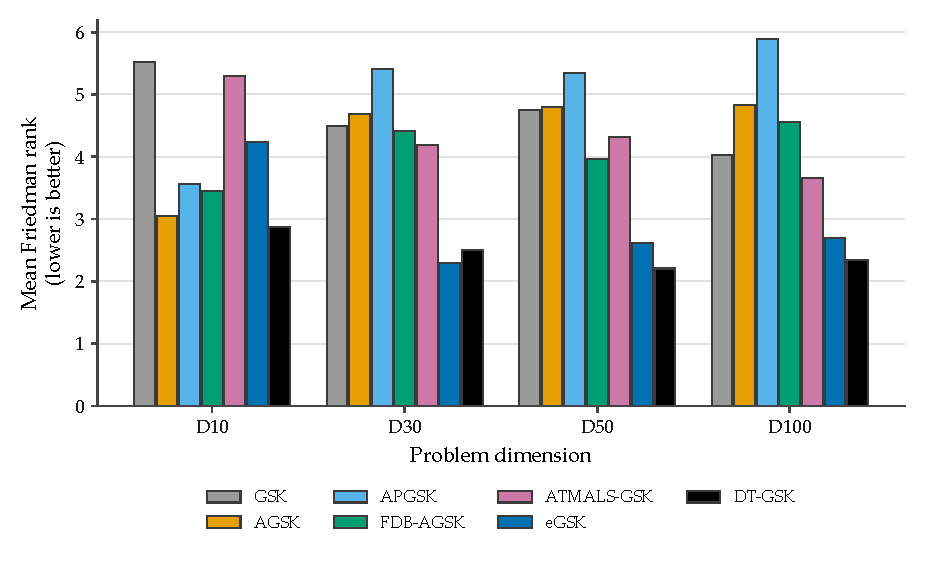
\includegraphics[width=0.75\textwidth]{figures/ranks/cec2017_mean_ranks.pdf}
\caption{Friedman mean ranks per dimension (CEC2017, 29 functions,
51 runs), grouped by dimension in the fixed panel order; companion to
Table~\ref{tab:friedman-cec2017}. Lower is better. Rank-robustness and APGSK-gap
qualifications as in Table~\ref{tab:friedman-cec2017}.}\label{fig:cec2017-ranks}
% BIND: FIG-CEC2017-RANKS (captions_registry)
\end{figure}

\subsubsection{Statistical Analysis}\label{sec:exp:stats}

\paragraph{Statistical protocol.}
Comparisons use the Wilcoxon signed-rank test~\cite{wilcoxon1945individual} on
paired per-function means, with Holm step-down
correction~\cite{holm1979simple} applied within each dimension over the family
of six comparators; the tie-corrected Friedman test~\cite{friedman1937use}
supplies mean ranks and Nemenyi critical differences supply the post-hoc
separation~\cite{demsar2006statistical}. In every case the null hypothesis is
that the compared algorithms' error distributions do not differ on the tested
family, and the alternative is that they do; $\alpha = 0.05$ throughout.
An effect size accompanies every test
--- the matched-pairs rank-biserial $r$ here, and BCa bootstrap intervals on the
mean ranks in the Supplementary Materials --- because a $p$-value alone does not
convey magnitude. Two reporting rules follow and are applied throughout. First,
an uncorrected family of per-comparator tests inflates the family-wise error
rate, so no significance claim in this paper rests on an uncorrected
$p$~\cite{holm1979simple,demsar2006statistical}. Second, win/tie/loss counts are
descriptive summaries of per-function outcomes and are never read as
significance: every $\alpha = 0.05$ decision reported here comes from a
Holm-adjusted test, and the two quantities are kept in separate columns so they
cannot be conflated.

Table~\ref{tab:wilcoxon-holm} reports the across-function Wilcoxon
tests with Holm correction, win/tie/loss counts, rank-biserial $r$ effect
sizes, and Holm decisions for \dtgsk{} against each comparator at
each dimension. Two qualifications apply to how that table should be
read. The companion $A_{12}$ summary is computed over the 29 per-function means,
on the same unit as the Wilcoxon test, and is therefore distinct from
the run-level $A_{12}$ reported in the effect-size workbook; the two
are not interchangeable. The \apgsk{} rows at
$D \in \{10, 30, 50\}$ rest on function-level tests over per-function
means, which was the inferential basis available there because \apgsk{}
per-run records were missing at analysis freeze and recovered only
afterwards.
% BIND: TAB-T15 (A12 unit-of-analysis; APGSK-GAP provenance)

\begin{table}[H]
\caption{\dtgsk{} vs.\ each GSK-family comparator on CEC2017 (29
functions, 51 runs, per-function mean error), in two aligned sub-tables:
$D \in \{10, 30\}$ above, $D \in \{50, 100\}$ below. Columns are the
across-function Wilcoxon signed-rank $p$ and its Holm-corrected value
(family $= 6$ comparators per dimension, $\alpha = 0.05$), win/tie/loss
counts with tie rule $|\Delta| < 10^{-8}$, the matched-pairs rank-biserial
effect size $r$ ($> 0$ favors \dtgsk{}), and the Holm decision ($+$ better,
$\approx$ no significant difference, $-$ worse).}\label{tab:wilcoxon-holm}
\centering
\tablesize{\footnotesize}
\setlength{\tabcolsep}{2.6pt}
\zebra
\begin{tabular}{lrrcccrcrrcccrc}
\toprule
\textbf{Algorithm} & \multicolumn{7}{c}{\textbf{D10}} & \multicolumn{7}{c}{\textbf{D30}} \\
 & $p$ & $p_{\mathrm{Holm}}$ & $+$ & $\approx$ & $-$ & $r$ & Dec. & $p$ & $p_{\mathrm{Holm}}$ & $+$ & $\approx$ & $-$ & $r$ & Dec. \\
\midrule
GSK & 0.0002 & 0.0010 & 22 & 4 & 3 & +0.865 & + & 0.0147 & 0.0295 & 19 & 2 & 8 & +0.540 & + \\
AGSK & 0.5422 & 1.0000 & 14 & 3 & 12 & -0.140 & = & 0.0026 & 0.0102 & 24 & 1 & 4 & +0.655 & + \\
APGSK & 0.9785 & 1.0000 & 16 & 4 & 9 & -0.009 & = & 0.0013 & 0.0064 & 24 & 0 & 5 & +0.687 & + \\
FDB-AGSK & 0.7639 & 1.0000 & 15 & 2 & 12 & -0.069 & = & 0.0009 & 0.0051 & 25 & 1 & 3 & +0.724 & + \\
ATMALS-GSK & 0.0091 & 0.0362 & 21 & 4 & 4 & +0.600 & + & 0.0035 & 0.0105 & 23 & 3 & 3 & +0.658 & + \\
eGSK & 0.0007 & 0.0035 & 21 & 4 & 4 & +0.778 & + & 0.1987 & 0.1987 & 11 & 2 & 16 & -0.286 & = \\
\bottomrule
\end{tabular}

\vspace{6pt}

\zebra
\begin{tabular}{lrrcccrcrrcccrc}
\toprule
\textbf{Algorithm} & \multicolumn{7}{c}{\textbf{D50}} & \multicolumn{7}{c}{\textbf{D100}} \\
 & $p$ & $p_{\mathrm{Holm}}$ & $+$ & $\approx$ & $-$ & $r$ & Dec. & $p$ & $p_{\mathrm{Holm}}$ & $+$ & $\approx$ & $-$ & $r$ & Dec. \\
\midrule
GSK & 0.0038 & 0.0075 & 22 & 0 & 7 & +0.618 & + & 0.0323 & 0.0646 & 20 & 0 & 9 & +0.457 & = \\
AGSK & 0.0002 & 0.0006 & 26 & 0 & 3 & +0.793 & + & $<$0.0001 & $<$0.0001 & 26 & 0 & 3 & +0.931 & + \\
APGSK & $<$0.0001 & 0.0003 & 27 & 0 & 2 & +0.857 & + & $<$0.0001 & $<$0.0001 & 28 & 0 & 1 & +0.977 & + \\
FDB-AGSK & 0.0002 & 0.0006 & 25 & 0 & 4 & +0.807 & + & $<$0.0001 & $<$0.0001 & 25 & 0 & 4 & +0.903 & + \\
ATMALS-GSK & 0.0001 & 0.0006 & 26 & 0 & 3 & +0.821 & + & 0.0005 & 0.0016 & 24 & 0 & 5 & +0.738 & + \\
eGSK & 1.0000 & 1.0000 & 13 & 0 & 16 & -0.002 & = & 0.7953 & 0.7953 & 12 & 0 & 17 & -0.057 & = \\
\bottomrule
\end{tabular}

% BIND: TAB-T15 (validated); captions_registry TAB-T15
\end{table}

Of the 24 Holm-corrected cells (six comparators $\times$ four
dimensions), 17 are significant wins for \dtgsk{}, 7 show no
significant difference, and none is a significant loss. The Holm correction is
applied within each dimension (family size 6), so this 24-cell count aggregates
four independent within-dimension families. It is a descriptive tally,
not a single jointly family-wise-error-controlled result.
% BIND: TAB-T15 (tally of the Dec. columns); Holm family = 6 per dimension (Sec. statistical protocol)
As a sensitivity check, applying Holm once across all 24 hypotheses --- the
most conservative reading, in which the four dimensions are treated as a
single family --- leaves 15 of the 24 cells significant. Only two cells do
not survive (\atmals{} at $D = 10$ and GSK at $D = 30$, both
$p_{\mathrm{Holm}}$ just under $0.05$ within their own dimension), and the
count of significant losses remains zero under either correction.
% BIND: AN-GHOLM-2017 (global_holm_sensitivity_cec2017.csv); M-028
The unfavorable and borderline cells are stated plainly. Against
\egsk{}, \dtgsk{} wins significantly only at $D = 10$
($p_{\mathrm{Holm}} = 0.0035$); at $D \in \{30, 50, 100\}$ the
outcome is not significant ($p_{\mathrm{Holm}} = 0.199$, $1.0$, and $0.795$)
with tabulated rank-biserial $r$ of $-0.286$, $-0.002$, and $-0.057$ ---
negligible magnitudes, all three faintly negative and therefore leaning
marginally toward \egsk{}.
% BIND: TAB-T15 (eGSK rows); negative_findings.md items 1, 3
Against GSK, the $D = 100$ cell is not significant after Holm correction
($p_{\mathrm{raw}} = 0.0323$, $p_{\mathrm{Holm}} = 0.0646$) despite a
20--0--9 win/tie/loss record.
% BIND: TAB-T15 (GSK row); negative_findings.md item 6
At $D = 10$, first place is carried by Holm-significant wins over
GSK, \atmals{}, and \egsk{} only; the cells against \agsk{},
\apgsk{}, and \fdbagsk{} show no significant difference
($p_{\mathrm{Holm}} = 1.0$ each).
% BIND: TAB-T15 (D10 columns); negative_findings.md item 5
At $D \in \{30, 50, 100\}$, \dtgsk{} beats \agsk{}, \apgsk{}, and
\fdbagsk{} in all nine cells ($p_{\mathrm{Holm}} \leq 0.011$) and
\atmals{} at all four dimensions
($p_{\mathrm{Holm}} \leq 0.037$); the largest effect is against
\apgsk{} at $D = 100$ ($r = +0.977$).
% BIND: TAB-T15 (AGSK/APGSK/FDB-AGSK/ATMALS-GSK rows)

Seeded bootstrap BCa rank-stability intervals attached to the Friedman mean ranks
(Supplementary Materials, Section~S2) qualify the rank point estimates. They
resample the fixed per-function midranks rather than recomputing ranks within
each resample, so they are read descriptively as a spread on the mean rank,
never as a formal overlap test. \dtgsk{}'s intervals are [2.29, 3.43], [2.07, 3.10],
[1.86, 2.69], and [1.90, 2.83] at $D = 10/30/50/100$; they overlap
\egsk{}'s intervals at $D \in \{30, 50, 100\}$, consistent with the
pairwise non-significant cells above.
% BIND: TAB-T16-BCA (papers/tables/T16_bca.tex; table typeset in the
% supplement only -- supplement scope per artifact_binding.csv; Phase 8
% assembly decision recorded in build_record.md)

Figure~\ref{fig:cd-cec2017} shows the Nemenyi mean-rank
plots with CD span (one panel per dimension), emitted only because the omnibus is significant at every
dimension; for $k = 7$ algorithms and $N = 29$ functions at
$\alpha = 0.05$, $\mathrm{CD} =
q_{0.05}\sqrt{k(k+1)/(6N)} = 1.67$ rank units
($q_{0.05} = 2.949$).
% BIND: nemenyi_cd_cec2017_D10.csv (CD = 1.672993, q = 2.949)
The plots make one limitation explicit: \dtgsk{} and \egsk{} are
never Nemenyi-separable at any CEC2017 dimension. Their rank gaps
are 1.36, 0.21, 0.41, and 0.34 at $D = 10/30/50/100$ on the unrounded mean
ranks, all inside the CD band. (The $D=100$ gap reads $0.35$ if formed from the
two-decimal displayed ranks.) The per-dimension orderings between these two
algorithms must therefore not be over-read as statistically established
separations.
% BIND: negative_findings.md item 4 (rank gaps vs CD)

\begin{figure}[htbp]
\centering
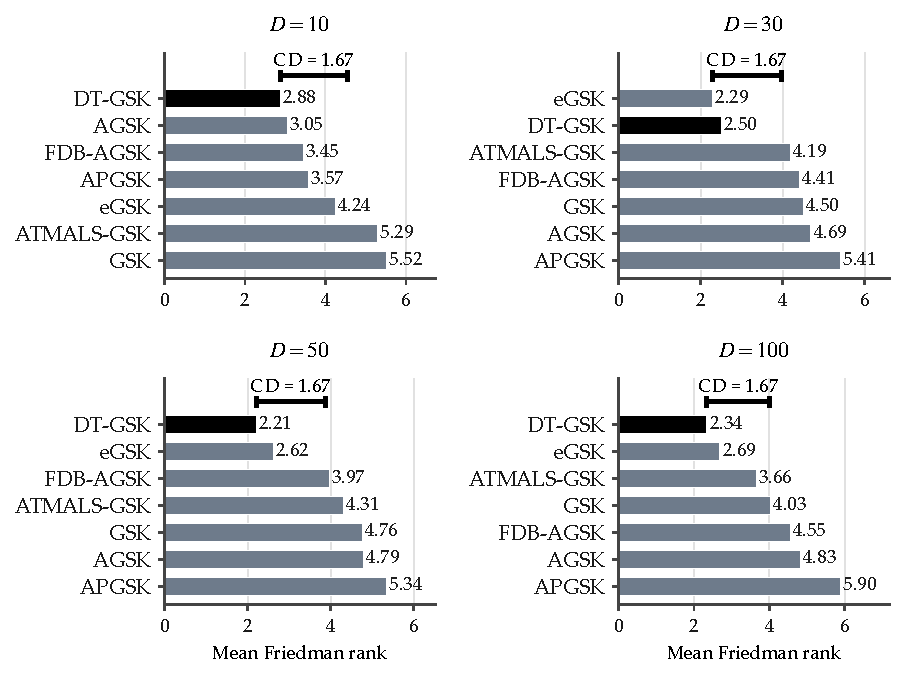
\includegraphics[width=\textwidth]{figures/nemenyi/nemenyi_cd_cec2017_grid.pdf}
\caption{Nemenyi mean-rank plots with critical-difference (CD) span for the
CEC2017 GSK-family Friedman mean ranks (lower is better), one panel per
dimension
($D = 10, 30, 50, 100$; $k = 7$, $N = 29$, $\alpha = 0.05$,
$\mathrm{CD} = 1.67$ rank units, $q_{0.05} = 2.949$); emitted only because the
Friedman omnibus is significant at every dimension.  The within-one-CD-of-best
cohort (the algorithms not separated from the best by more than one CD) is
\{\dtgsk{}, \agsk{}, \fdbagsk{}, \apgsk{}, \egsk{}\} at $D{=}10$;
\{\egsk{}, \dtgsk{}\} at $D{=}30$ (best rank \egsk{}); \{\dtgsk{}, \egsk{}\}
at $D{=}50$; and \{\dtgsk{}, \egsk{}, \atmals{}\} at $D{=}100$.  Rank-robustness
and APGSK-gap qualifications as in
Table~\ref{tab:friedman-cec2017}.}\label{fig:cd-cec2017}
% BIND: FIG-CD-D10/D30/D50/D100 (captions_registry; consolidated 2x2 grid image)
\end{figure}

The Friedman mean rank improves with dimension overall but is not monotone
across $D \in \{10, 30, 50, 100\}$ --- 2.88, 2.50, 2.21, 2.34 ---: $D = 30$
is an ordinal dip to second place and $D = 100$ is slightly worse than
$D = 50$ (a rank-versus-dimension trend plot is provided in the Supplementary
Materials).
% BIND: AN-TREND-2017 (rank_trend_cec2017.csv); negative_findings.md item 9

\paragraph{Robustness of the rank statements.}
A prespecified robustness battery accompanies the release, and two
of its checks diverge from the primary analysis and therefore qualify
every rank-ordering statement above. Re-ranking on median (rather
than mean) per-function errors shifts win/tie/loss tallies materially
--- 21--4--4 becomes 17--10--2 against \egsk{} at $D = 10$ --- and
swaps two comparator pairs, \apgsk{}/\egsk{} at $D = 10$ and
\fdbagsk{}/\atmals{} at $D = 50$. Excluding the disputed APGSK cells
at $D \leq 50$ swaps GSK and \fdbagsk{} at $D = 30$.
% BIND: AN-ROB-2017-01, AN-ROB-2017-04 (robustness_cec2017_r01/r04*.csv; negative_findings.md item 7)
Mean-based ranks are the prespecified primary; \dtgsk{}'s own
ordinal positions (1/2/1/1 at $D = 10/30/50/100$) are identical in
every variant reported here, but panel orderings between comparators are not fully
robust. Under the median endpoint \dtgsk{}'s $D = 100$ first place becomes
an exact tie with \egsk{} (both 2.59), consistent with their documented
non-separability. As a deliberate pairing-sensitivity check, an unpaired Mann--Whitney companion was also run over the
696 function-by-comparator-by-dimension cells, each a run-level test on 51
paired runs. Dropping the pairing moves 11 cells from significant to
non-significant and 21 in the opposite direction, with no sign reversals. The
robustness criterion (no sign reversals) is met, and the net effect of
dropping the pairing is an increase in significances rather than a
simple power loss --- and an
exploratory Benjamini--Hochberg
companion~\cite{benjamini1995controlling} over the run-level tests is
included in the released analysis workbooks (which accompany the
reproducibility bundle, not the typeset supplement).
One robustness check is disclosed as a surrogate. Because errors are floored
to zero at write time, raw sub-floor values are unrecoverable from the
release, so the error-floor sensitivity check could not be run on the raw
values. It was executed instead in its pre-registered nearest-admissible form,
with ties handled at the floor and means $\le 10^{-8}$ snapped to zero before
ranking and win/tie/loss. A scan of the 71,400 stored per-run errors found no
value in the open interval $(0, 10^{-8})$, so the surrogate and the raw check
would coincide on this release. The substitution is nonetheless recorded rather
than presented as the check itself.
% BIND: AN-ROB-2017-05 (r05 unpaired companion); AN-EXP-BH-2017; AN-ROB-2017-02 (r02 branch-B surrogate disclosure)

%------------------------------------------------------------------
\subsection{Results on the CEC2011 Real-World Suite}\label{sec:exp:cec2011}
%------------------------------------------------------------------

The per-problem five-statistic results of \dtgsk{} against the original
GSK on the 22 CEC2011 problems --- together with the \egsk{} loss and the
\dtgsk{}-versus-GSK detail --- are reported in the Supplementary Materials,
Section~S2 (the complete six-comparator across-problem Wilcoxon--Holm
matrix is in the released analysis bundle), and the full convergence grids
in Section~S3. The endpoint is the raw best objective value; error cells
are NaN by design on problems without published optima, and best-fitness
is authoritative there. This suite is corroborative, so the main text
reports its ranking (Figure~\ref{fig:cec2011-ranks}) and significance
below and defers the dense per-problem five-statistic table to the
supplement.
% BIND: PR-02 (claims matrix); TAB-T01 relocated to Supplement S2 (M028 density)

Within the GSK-family panel, \dtgsk{} places second of seven on
CEC2011 by Friedman mean rank (3.36), behind \egsk{} (2.52); the
omnibus is significant (Iman--Davenport $F = 4.27$,
$p = 6.0 \times 10^{-4}$), and Figure~\ref{fig:cec2011-ranks} shows
the resulting ordering.
% BIND: AN-OMNI-2011-NATIVE (friedman_ranks_cec2011.csv); RS-10 ACCEPTED wording
The across-problem Holm-corrected Wilcoxon against \egsk{} is a
statistically significant loss
($p_{\mathrm{raw}} = 9.5 \times 10^{-3}$,
$p_{\mathrm{Holm}} = 4.2 \times 10^{-2}$). It is the single
Holm-significant unfavorable headline cell in this study, and it
accompanies every CEC2011 placement statement in this paper. As on CEC2017,
the \dtgsk{}--\egsk{} Friedman-rank gap of $0.84$ is nonetheless within the
Nemenyi critical difference of $1.92$ here.
% BIND: AN-PW-2011-NATIVE (wilcoxon_holm_cec2011.csv, egsk row); negative_findings.md item 2
The remaining pairwise outcomes at the same family size are two
significant wins --- against \agsk{}
($p_{\mathrm{Holm}} = 1.6 \times 10^{-2}$) and \fdbagsk{}
($p_{\mathrm{Holm}} = 4.2 \times 10^{-2}$) --- and no significant difference against GSK,
\apgsk{} ($p_{\mathrm{Holm}} = 0.137$ each), and \atmals{}
($p_{\mathrm{Holm}} = 0.323$).
% BIND: AN-PW-2011-NATIVE (wilcoxon_holm_cec2011.csv all rows)
The head-to-head against the original GSK illustrates why the suite
is corroborative rather than headline evidence: the descriptive
record favors \dtgsk{} (win/tie/loss 13--2--7,
$R^{+} = 159$ vs.\ $R^{-} = 51$), but the across-problem test does
not survive Holm correction
($p_{\mathrm{raw}} = 4.6 \times 10^{-2}$,
$p_{\mathrm{Holm}} = 0.137$) at $n = 22$ problems.
% BIND: TAB-T06 (papers/tables/T06.tex; R+, R-, p, p_holm, W/T/L)
CEC2011 therefore corroborates within-family competitiveness on
real-world problems at native dimensions --- a competitive placement
(second of seven) --- and does not corroborate first place; no headline
claim in this paper rests on CEC2011 alone.
% BIND: IN-03 NARROWED (claims matrix)

\begin{figure}[H]
\centering
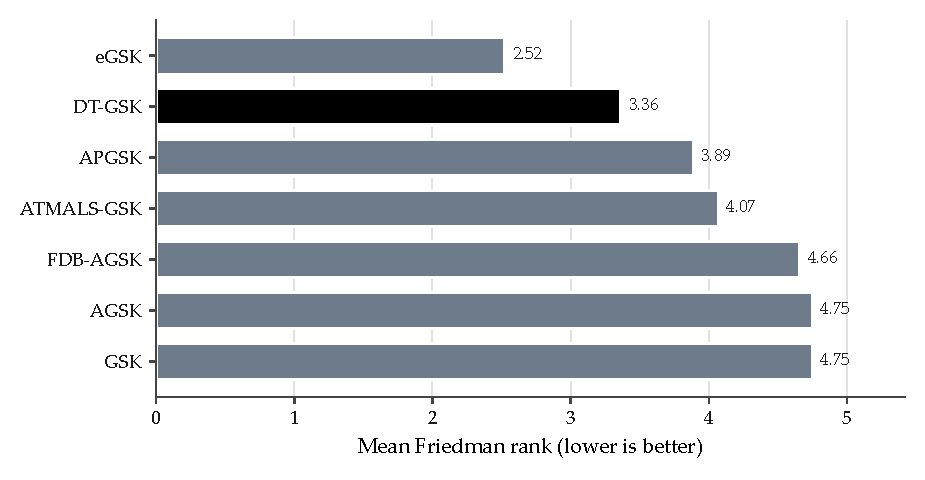
\includegraphics[width=0.70\textwidth]{figures/ranks/cec2011_ranks.pdf}
\caption{Friedman mean ranks over the 22 CEC2011 real-world problems
(25 runs each, raw best-fitness basis), sorted best-first; \dtgsk{}
highlighted. Lower is better. 
Within this panel \dtgsk{}'s across-problem Wilcoxon vs.\ \egsk{} is
a significant loss (Holm $p = 4.2 \times 10^{-2}$).}\label{fig:cec2011-ranks}
% BIND: FIG-CEC2011-RANKS (captions_registry) [CEC2011-EGSK-LOSS]
\end{figure}

%------------------------------------------------------------------
\subsection{Results on the CEC2013 Second Comparison Suite}\label{sec:exp:cec2013}
%------------------------------------------------------------------

CEC2013 is reported as a second comparison suite --- for breadth of
comparison under the identical protocol --- and carries no
independence claim of any kind. The per-function five-statistic
tables and the Wilcoxon summaries are in the Supplementary Materials,
Section~S2; the panel-level numbers quoted here are re-derivable from
the released analysis bundle.
% BIND: PR-03, RS-11 (claims matrix)

Within the GSK-family panel, \dtgsk{} attains the best overall
Friedman mean rank on CEC2013 (2.80, unweighted mean of the three
per-dimension mean ranks, the same descriptive convention as
Table~\ref{tab:friedman-cec2017}; \egsk{} is second at 3.41).
Table~\ref{tab:friedman-cec2013} reports the full per-dimension panel.
% BIND: AN-RANKAGG-2013-OVERALL (friedman_ranks_cec2013_overall.csv)

\begin{table}[H]
\caption{Friedman mean ranks (lower is better) of the seven-algorithm
GSK-family panel on the CEC2013 second comparison suite per dimension
(28 per-function mean errors as blocks, 51 runs each) plus the
unweighted across-dimension mean (``Overall'', a descriptive
aggregate); the Friedman + Iman--Davenport omnibus is significant at
every dimension ($p \leq 1.1 \times 10^{-3}$). Best rank per column in
bold. CEC2013 is reported for breadth of comparison and carries no
independence claim. }\label{tab:friedman-cec2013}
\centering
\tablesize{\footnotesize}
\zebra
\begin{tabular}{lcccc}
\toprule
\textbf{Algorithm} & \textbf{D10} & \textbf{D30} & \textbf{D50} & \textbf{Overall} \\
\midrule
GSK & 5.88 & 4.98 & 5.16 & 5.34 \\
\agsk{} & 3.80 & 4.48 & 4.52 & 4.27 \\
\apgsk{} & 3.88 & 4.63 & 4.79 & 4.43 \\
\fdbagsk{} & 3.95 & 4.13 & 4.27 & 4.11 \\
\atmals{} & 4.21 & 3.34 & 3.38 & 3.64 \\
\egsk{} & 3.88 & \textbf{3.07} & 3.29 & 3.41 \\
\dtgsk{} & \textbf{2.41} & 3.38 & \textbf{2.61} & \textbf{2.80} \\
\bottomrule
\end{tabular}
% BIND: AN-RANKAGG-2013-OVERALL (friedman_ranks_cec2013_overall.csv); AN-OMNI-2013-D10/D30/D50 (friedman_ranks_cec2013_D{10,30,50}.csv); PR-03 (second comparison suite; no independence claim)
\end{table}

The per-dimension picture is first/third/first: at $D = 10$,
\dtgsk{} leads with mean rank 2.41 (omnibus
$p = 5.3 \times 10^{-8}$); at $D = 30$ it places \emph{third} (3.38)
behind \egsk{} (3.07) and \atmals{} (3.34) (omnibus
$p = 1.1 \times 10^{-3}$); at $D = 50$ it leads again with 2.61
(omnibus $p = 2.9 \times 10^{-6}$).
% BIND: AN-OMNI-2013-D10/D30/D50 (friedman_ranks_cec2013_D*.csv); negative_findings.md item 10
The $D = 30$ third place is disclosed as this suite's counterpart of
the CEC2017 mid-dimension weakness; the across-function
Holm-corrected Wilcoxon tests at $D = 30$ against both \egsk{} and
\atmals{} show no significant difference ($p_{\mathrm{Holm}} = 0.748$
each), so the deficit is ordinal, not statistically separable.
% BIND: AN-PW-2013-D30 (wilcoxon_holm_cec2013_D30.csv, egsk/atmals rows)
Against the original GSK, \dtgsk{} records Holm-significant wins at
all three dimensions
($p_{\mathrm{Holm}} = 1.9 \times 10^{-4}$, $3.1 \times 10^{-2}$, and
$2.7 \times 10^{-3}$ at $D = 10/30/50$; win/tie/loss 24--2--2,
21--2--5, and 24--2--2; $R^{+}/R^{-} = 340/11$, $286/65$, and
$314/37$).
% BIND: TAB-T14 (papers/tables/T14.tex); AN-PW-2013-D10/D30/D50
The dimension profile of these outcomes mirrors the primary suite:
the mid-dimension tier is where the improved family variants ---
\egsk{} and \atmals{} in particular --- are hardest to separate,
while the low- and upper-dimension tiers favor \dtgsk{} within the
panel.
% BIND: AN-OMNI-2013-D10/D30/D50 (ordinal reading of friedman_ranks_cec2013_D*.csv)
Because these results come from the same protocol and pairing as the
primary suite, they are read as breadth of comparison within the GSK
family panel, not as evidence of generalization beyond the suites
tested.
% BIND: RS-11 permitted wording

%------------------------------------------------------------------
\subsection{Results on the CEC2020 Pre-Registered Confirmatory Suite}\label{sec:exp:cec2020}
%------------------------------------------------------------------

CEC2020 is the one suite in this study whose entire analysis --- the
hypotheses, the analysis families, the tie rules, and the three candidate
outcome sentences --- was committed to the repository before any CEC2020
result existed, at the signing commit 5c9bfae82 of the registered
analysis-plan addendum. The complete registered battery, its robustness
checks, and the mid-campaign inspection ledger are reported in
Supplementary Section~S8, and the outcome sentence below is the
pre-committed wording-bank variant selected by the data, not re-drafted
after the fact.
% BIND: SAP addendum Sections 3-4, 9, 13 (signing commit 5c9bfae82, before any CEC2020 datum); Amendment 2 A2.3
The protocol is the registered one of Table~\ref{tab:protocol}: 10
functions at $D \in \{5, 10, 15, 20\}$, with F6 and F7 undefined at
$D = 5$ (38 scored cells), 30 runs per cell, a MaxFES that rises from
$5 \times 10^{4}$ at $D = 5$ to $10^{7}$ at $D = 20$, and the error
basis with the $10^{-8}$ floor.
% BIND: SAP addendum Section 2 (registered protocol facts); yue2020cec2020

On AGSK's strongest suite --- the CEC2020 competition in which it was
the runner-up~\cite{apgsk2021} --- \dtgsk{} places fourth; the family
panel corroborates AGSK's published strength in this regime, consistent
with the tiering thesis: every dimension-gated \dtgsk{} subsystem is
inactive at $D \leq 20$.
% BIND: RS-12 (SAP addendum Sec. 9 [AGSK first] variant verbatim, slot = fourth per Amendment 2 A2.3, factual clause corrected per Amendment 3 A3.2); friedman_ranks_cec2020_overall.csv (dt-gsk ordinal 4)
The descriptive across-dimension aggregate (the unweighted mean of the
four per-dimension Friedman mean ranks; no test is attached, the $D = 5$
task set is reduced to 8 functions, and MaxFES changes by dimension, so
the aggregate mixes budget regimes) is 4.11 for \dtgsk{}, fourth of
seven; \agsk{} is best at 2.09, \fdbagsk{} second at 2.31, and \apgsk{}
third at 3.09.
% BIND: AN-RANKAGG-2020-OVERALL (friedman_ranks_cec2020_overall.csv)
Per dimension, the Friedman--Iman--Davenport omnibus separates the panel
at every dimension ($p \leq 6.1 \times 10^{-5}$), with the registered
seeded permutation check agreeing at each; the mean ranks place \dtgsk{}
at 4.25 (fourth) at $D = 5$, 4.10 (fourth) at $D = 10$, 3.50 (tied-third
with \apgsk{}) at $D = 15$, and 4.60 (fifth) at $D = 20$, while \agsk{}
holds the best mean rank at $D \in \{10, 15, 20\}$ (1.90, 2.10, 1.60)
and \apgsk{} at $D = 5$ (2.38).
Table~\ref{tab:cec2020-ranks} reports the complete panel.
% BIND: AN-OMNI-2020-D5/D10/D15/D20 (friedman_ranks_cec2020_5.csv, friedman_ranks_cec2020_10.csv, friedman_ranks_cec2020_15.csv, friedman_ranks_cec2020_20.csv)

\begin{table}[H]
\caption{CEC2020 final panel results: tie-corrected Friedman mean ranks per
dimension (lower is better; 30 runs per cell, error basis with the $10^{-8}$
floor) and the descriptive across-dimension aggregate. No test is attached to
the aggregate: the $D=5$ task set is reduced to 8 functions (F6 and F7 are
undefined there), and MaxFES changes with dimension, so the aggregate mixes
budget regimes. The omnibus rows give the tie-corrected Friedman statistic,
the Iman--Davenport $p$, and the registered seeded permutation $p$
($B = 10^{5}$). Per-dimension ranks are exact at three decimals ($N$ = 8 or
10); the aggregate, their unweighted mean, is printed at four. Per-function
detail, run-level tests, and effect sizes are in Supplementary
Section~S8.}\label{tab:cec2020-ranks}
\centering
\tablesize{\footnotesize}
\setlength{\tabcolsep}{5pt}%
\begin{tabular}{lccccc}
\toprule
\textbf{Algorithm} & $\bm{D=5}$ & $\bm{D=10}$ & $\bm{D=15}$ & $\bm{D=20}$ & \textbf{Aggregate} \\
\midrule
\agsk{} & 2.750 & \bestval{1.900} & \bestval{2.100} & \bestval{1.600} & \bestval{2.0875} \\
\fdbagsk{} & 2.750 & 2.200 & 2.300 & 2.000 & 2.3125 \\
\apgsk{} & \bestval{2.375} & 3.000 & 3.500 & 3.500 & 3.0938 \\
\dtgsk{} & 4.250 & 4.100 & 3.500 & 4.600 & 4.1125 \\
\egsk{} & 4.875 & 5.400 & 5.500 & 6.000 & 5.4437 \\
GSK & 5.625 & 6.200 & 5.500 & 4.500 & 5.4562 \\
\atmals{} & 5.375 & 5.200 & 5.600 & 5.800 & 5.4938 \\
\midrule
Functions ($N$) & 8 & 10 & 10 & 10 & --- \\
Friedman $\chi^{2}$ (tie-corr.) & 23.22 & 40.24 & 37.66 & 42.52 & --- \\
Iman--Davenport $p$ & $6.1\times10^{-5}$ & $1.8\times10^{-11}$ & $4.3\times10^{-10}$ & $7.2\times10^{-13}$ & --- \\
Permutation $p$ & $7.0\times10^{-5}$ & $1.0\times10^{-5}$ & $1.0\times10^{-5}$ & $1.0\times10^{-5}$ & --- \\
\bottomrule
\end{tabular}
% BIND: AN-OMNI-2020-D5/D10/D15/D20 + AN-RANKAGG-2020-OVERALL
% (friedman_ranks_cec2020_5.csv, friedman_ranks_cec2020_10.csv,
%  friedman_ranks_cec2020_15.csv, friedman_ranks_cec2020_20.csv,
%  friedman_ranks_cec2020_overall.csv; permutation seed
%  SeedSequence([20240620, 2020, dim, 0, 99]), B=100000)
\end{table}
In the registered across-function pairwise layer, \dtgsk{} is
Holm-separated in five of the twenty-four comparator--dimension cells:
three favorable --- against \atmals{} and \egsk{} at $D = 15$, and
against \egsk{} at $D = 20$ --- and two unfavorable --- against \agsk{}
and \fdbagsk{} at $D = 20$. In the remaining nineteen cells, including
every comparison at $D = 5$ and $D = 10$, no separation is demonstrated.
% BIND: AN-PW-2020-D5..D20 (wilcoxon_holm_cec2020_5.csv, wilcoxon_holm_cec2020_10.csv, wilcoxon_holm_cec2020_15.csv, wilcoxon_holm_cec2020_20.csv)
This fourth place is the boundary finding that the registered directional
expectation predicted in advance --- \agsk{} and \apgsk{} favored on
their home regime, every dimension-gated \dtgsk{} subsystem structurally
off at $D \leq 20$ --- and it is reported as such, not as a result that
``does not count''; no CEC2020 sentence in this paper claims superiority
over \agsk{} or \fdbagsk{} at any dimension.
% BIND: SAP addendum Section 3 (directional expectation); Amendment 2 A2.3 (binding wording constraints)
One conflict adjacency accompanies every interpretation of this suite,
here as in the back matter: \agsk{} was the runner-up of the CEC2020
competition~\cite{apgsk2021}, and its paper is a co-author's.
% BIND: SAP addendum Section 10 (conflict-adjacency disclosure, factual clause corrected per Amendment 3 A3.2); RS-12

%------------------------------------------------------------------
\subsection{Results on the CEC2013LSGO Large-Scale Suite}\label{sec:exp:cec2013lsgo}
%------------------------------------------------------------------

The CEC2013LSGO analysis in this paper is family-internal: it ranks the
seven GSK-family variants against one another under a common protocol.
Dedicated large-scale optimizers --- for example
SHADE-ILS~\cite{molina2018shadeils} and MOS~\cite{latorre2013mos} ---
report substantially stronger published results on this suite than any
GSK-family member, and no competitiveness with such specialists is
claimed here; cross-paradigm comparison is outside this paper's scope.
% BIND: FINAL_PUBLICATION_PLAN.md 0.4 sentence (a), adopted verbatim; LM-06; RS-13
The suite's evidential tier is disclosed rather than implied: the
descriptive layer (mean ranks, omnibus, win/tie/loss) was inspected
informally before the analysis addendum was signed and therefore carries
no confirmatory weight, whereas the run-level paired layer had never
been computed before registration and is confirmatory-with-disclosure;
both are reported in full, with this provenance, in Supplementary
Section~S7.
% BIND: SAP addendum Section 6 (prior-inspection disclosure); Amendment 1 A1.3

Descriptively, \dtgsk{} and \agsk{} share the best family mean rank
(tied-first, 3.13 each, over the 15 function blocks); no member except
\egsk{} (worse, at 5.47) is separable by the omnibus procedure at the
Nemenyi critical distance of 2.33, and \dtgsk{} is last on F7 and F15.
Table~\ref{tab:lsgo-ranks} reports the final family panel.
% BIND: AN-OMNI-LSGO-NATIVE (friedman_ranks_cec2013lsgo_native.csv; nemenyi_cd_cec2013lsgo_native.csv); registered claim ceiling (SAP addendum Section 9)

\begin{table}[H]
\caption{CEC2013LSGO final family panel: tie-corrected Friedman mean ranks
over the 15 function blocks (raw best-objective basis, 25 runs per cell;
lower is better) with the across-function Wilcoxon layer against \dtgsk{}
(win--tie--loss on per-function means, tie band $10^{-8}$; exact
two-sided sign-flip $p$; Holm-adjusted over the six comparators). The
descriptive columns carry no confirmatory weight (inspected before
registration); the pairwise columns are the registered
supporting-with-disclosure layer, and no comparator separates from
\dtgsk{}. An exact rank tie is reported as tied-first, never absorbed.
Omnibus: Friedman $\chi^{2} = 15.31$, Iman--Davenport $p = 0.014$;
Nemenyi critical distance $2.33$ ($k = 7$, $N = 15$). Run-level tests and
effect sizes are in Supplementary Section~S7.}\label{tab:lsgo-ranks}
\centering
\tablesize{\footnotesize}
\setlength{\tabcolsep}{5pt}%
\begin{tabular}{lccccc}
\toprule
\textbf{Algorithm} & \textbf{Mean rank} & \textbf{Ordinal} &
\textbf{\dtgsk{} W--T--L} & \textbf{Exact} $\bm{p}$ & \textbf{Holm} $\bm{p}$ \\
\midrule
\dtgsk{} & \bestval{3.133} & 1 (tied-first) & --- & --- & --- \\
\agsk{} & \bestval{3.133} & 1 (tied-first) & 9--0--6 & 0.8469 & 1.0000 \\
\atmals{} & 3.533 & 3 & 8--0--7 & 0.1688 & 0.5065 \\
GSK & 3.867 & 4 & 8--0--7 & 0.7615 & 1.0000 \\
\fdbagsk{} & 3.933 & 5 & 11--0--4 & 0.0833 & 0.3330 \\
\apgsk{} & 4.933 & 6 & 11--0--4 & 0.0554 & 0.2875 \\
\egsk{} & 5.467 & 7 & 11--0--4 & 0.0479 & 0.2875 \\
\bottomrule
\end{tabular}
% BIND: AN-OMNI-LSGO-NATIVE + AN-PW-LSGO-NATIVE
% (friedman_ranks_cec2013lsgo_native.csv; nemenyi_cd_cec2013lsgo_native.csv
%  q=2.949, CD=2.326203; wilcoxon_holm_cec2013lsgo_native.csv -- W-T-L stated
%  as dt-gsk wins-ties-losses per comparator row)
\end{table}
The registered paired layers resolve the standing: across functions, no
comparator separates from \dtgsk{} after Holm correction, and in
particular the paired tests do not separate \dtgsk{} from \agsk{} (exact
$p = 0.847$, Holm-adjusted $1.0$) --- the registered ceiling wording,
tied-first descriptive rank with no paired separation, applies verbatim.
% BIND: AN-PW-LSGO-NATIVE (wilcoxon_holm_cec2013lsgo_native.csv, agsk row); Amendment 1 A1.3 (binding wording consequence)
At run level the picture is regular in both directions, and both are
stated: \dtgsk{} is Holm-significantly better than every one of the six
family members on F4 and F8, and Holm-significantly worse than every one
of them on F7 and F15.
% BIND: AN-PWRUN-LSGO-NATIVE (wilcoxon_run_cec2013lsgo_native.csv: F4/F8 win vs all six comparators; F7/F15 loss vs all six)
The effect layer bars any superiority reading against \atmals{}: the
mean run-level effect across the 15 functions marginally favors that
comparator (mean Cliff's delta $-0.0025$ against \dtgsk{}), so the
effect layer supports no superiority claim over \atmals{} on this suite.
% BIND: AN-EFF-LSGO-NATIVE (effect_sizes_cec2013lsgo_native.csv, atmals-gsk rows; mean of the 15 cliffs_delta cells = -0.002453)
The one \dtgsk{}-specific configuration addition on this suite --- the
two linkage-block-size entries for $D = 905$ and $D = 1000$ described in
Section~\ref{sec:exp:settings} --- is disclosed, with its rule,
rationale, and timing, in Supplementary Section~S7.
% BIND: production_deviation_record.md D-8.4

%------------------------------------------------------------------
\subsection{Convergence Analysis}\label{sec:exp:convergence}
%------------------------------------------------------------------

Figures~\ref{fig:conv-cec2017-d30} and~\ref{fig:conv-cec2017-d100}
show family-overlay convergence curves on CEC2017 at the two featured
dimensions. The function selection was prespecified and frozen
before rendering, stratified over function category, difficulty tercile, and
\dtgsk{} standing, and it deliberately includes an unfavorable case.
At $D = 30$ the selected panel comprises F3 (unimodal, easy/strong),
F10 (simple multimodal, hard/comparable), F12 (hybrid, hard/comparable),
and F26 (composition, hard/weak --- the mandated unfavorable case).
At $D = 100$ it comprises F1 (unimodal, easy/strong),
F5 (simple multimodal, easy/strong), F12 (hybrid, hard/comparable),
and F26 (composition, hard/comparable).
% BIND: AN-CONV-2017-D30/D100 (curve_selection_cec2017_D30.csv, curve_selection_cec2017_D100.csv)
Every curve is the per-checkpoint \emph{mean} error across all 51
runs of that algorithm --- the identical aggregation basis for all
seven curves in every panel, with no smoothing and no
interpolation --- on a log-error axis whose display-only floor of
$10^{-14}$ marks exact zeros and never enters any statistic. The
complete convergence sets --- CEC2017 at all four dimensions, CEC2011
at native dimensions, and CEC2013 at the prespecified $D = 30$ --- are
in the Supplementary Materials, Section~S3.
% BIND: captions_registry conventions (aggregation, display floor)

The unfavorable case is discussed rather than skipped. On F26 at
$D = 30$, \dtgsk{}'s final mean error ($1.16 \times 10^{3}$) is
higher than five of the six comparators; only \atmals{}
($1.32 \times 10^{3}$) ends higher. Its best run
($9.85 \times 10^{2}$) never reaches the low attractor that every
comparator's best run reaches ($2.00$--$3.00 \times 10^{2}$). At the
same time its standard deviation ($7.5 \times 10^{1}$) is the
smallest in the panel, the next smallest being GSK's
$2.7 \times 10^{2}$.
% BIND: AN-DESC-2017-D30 (descriptive_stats_cec2017_D30.csv, F26 rows)
The measured pattern at this cell is thus consistent mid-level
convergence without basin escapes, on a composition function at the
dimension where the structure-memory subsystems are inactive
(Section~\ref{sec:algorithm}); per-component attribution is not
claimed.
% BIND: LM-02 (claims matrix; gating stated as design fact)
At $D = 100$ the same function is a comparable case: \dtgsk{}'s
final mean error ($4.09 \times 10^{3}$) sits below four comparators
(\atmals{} $5.55 \times 10^{3}$; \fdbagsk{} $1.03 \times 10^{4}$;
\agsk{} $1.10 \times 10^{4}$; \apgsk{} $1.22 \times 10^{4}$) and
above GSK ($3.69 \times 10^{3}$) and \egsk{}
($3.05 \times 10^{3}$).
% BIND: AN-DESC-2017-D100 (descriptive_stats_cec2017_D100.csv, F26 rows)

\begin{figure}[H]
\centering
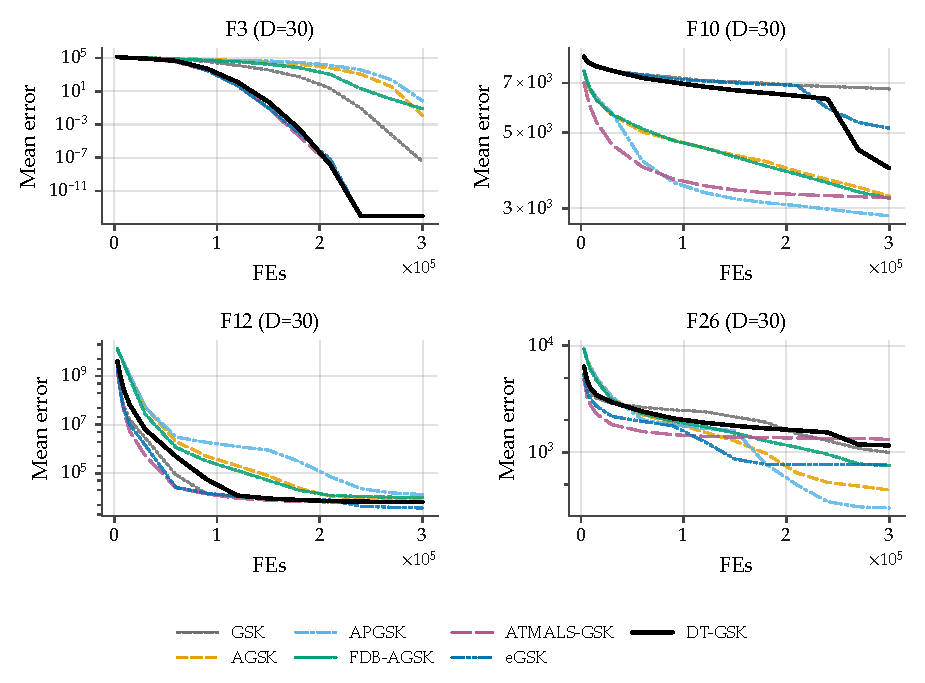
\includegraphics[width=0.92\textwidth]{figures/convergence/main_cec2017_D30.pdf}
\caption{Family-overlay convergence on CEC2017 at $D = 30$ for the
four functions selected by a fixed, prespecified rule and frozen before rendering:
F3 (unimodal; easy/strong), F10 (simple multimodal;
hard/comparable), F12 (hybrid; hard/comparable), F26 (composition;
hard/weak --- the mandated unfavorable case). Each panel overlays all
7 panel algorithms; every curve is the per-checkpoint mean error
across 51 runs (identical basis; no smoothing); log-error $y$-axis
with a display-only floor of $10^{-14}$ for exact zeros (never enters
any statistic); one shared legend. $D = 30$ is \dtgsk{}'s known-weak
tier: rank \#2 behind \egsk{}. 
APGSK checkpoint evidence at $D = 30$ carries the per-run availability
qualification of
Section~\ref{sec:exp:settings}.}\label{fig:conv-cec2017-d30}
% BIND: FIG-CONV-MAIN-D30 (captions_registry)
\end{figure}

\begin{figure}[H]
\centering
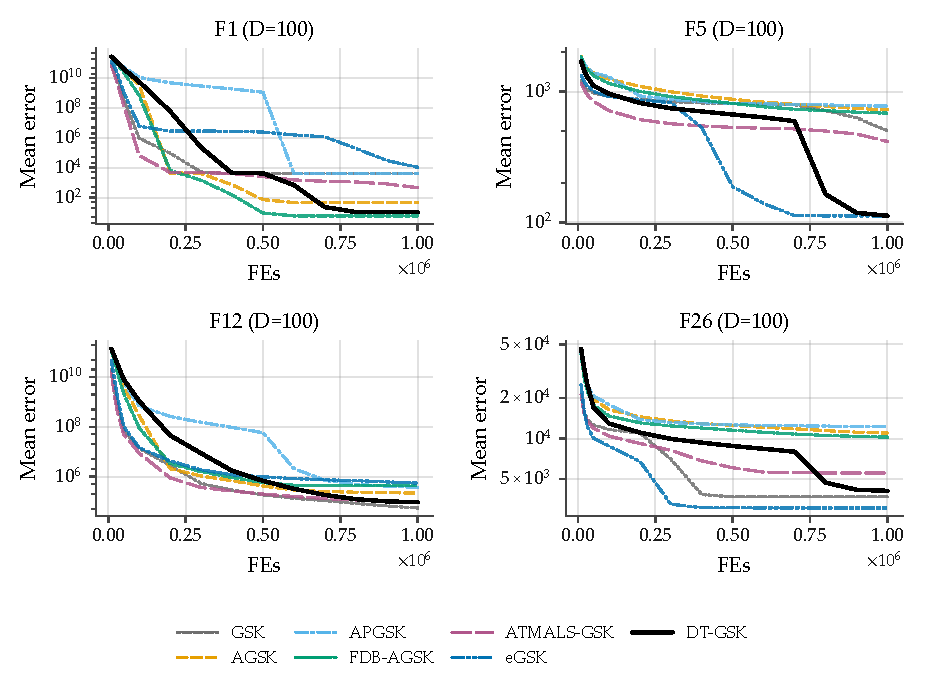
\includegraphics[width=0.92\textwidth]{figures/convergence/main_cec2017_D100.pdf}
\caption{Family-overlay convergence on CEC2017 at $D = 100$ (tier
where the structure-memory and polish subsystems are active) for the
four prespecified functions: F1 (unimodal; easy/strong), F5 (simple
multimodal; easy/strong), F12 (hybrid; hard/comparable), F26
(composition; hard/comparable). Per-checkpoint mean error across 51
runs per algorithm, 7-curve overlay, log-error $y$-axis (display
floor $10^{-14}$), one shared legend. }\label{fig:conv-cec2017-d100}
% BIND: FIG-CONV-MAIN-D100 (captions_registry)
\end{figure}

%------------------------------------------------------------------
\subsection{Runtime and Complexity in Practice}\label{sec:exp:runtime}
%------------------------------------------------------------------

Table~\ref{tab:runtime} reports \dtgsk{}'s measured per-run wall-clock time on
CEC2017 (mean $\pm$ SD over the 1{,}479 runs per dimension cell, i.e., 29
functions $\times$ 51 runs), collected in a single environment: the 51-run
post-fix campaign with the interaction graph's compiled kernels active. The
comparator timings were collected in a separate measurement session, so we do
not tabulate a cross-algorithm wall-clock comparison and make no
runtime-superiority claim; the figures characterize \dtgsk{}'s own cost.
% BIND: AN-COST-2017 (cost_cec2017.csv, dt-gsk cec2017 rows); LM-04

\dtgsk{}'s per-run time scales with dimension, from 4.93~s at $D = 10$ to
41.59~s at $D = 100$ --- the bookkeeping cost of its scaffold and
structure-memory subsystems on top of the unchanged GSK vector-update operator. These are
measured costs at matched evaluation budgets: the overhead is bookkeeping, not
extra objective evaluations (Section~\ref{sec:algorithm}), and it grounds the
overhead limitation restated in the conclusions. These measurements are the
empirical counterpart of the per-tier asymptotic cost model in
Section~\ref{sec:alg:complexity}, so cost is reported both analytically and in
wall-clock terms. The isolated compute cost of
the interaction-structure memory is quantified in the Supplementary Materials
(Section~S6.5; the measurement provenance for those figures is recorded in
Section~S6.7). On the other suites \dtgsk{}'s mean per-run time is
4.45--34.26~s across CEC2013 $D \in \{10, 30, 50\}$ and 80.64~s on CEC2011
(native dimensions). No comparator wall-clock is reported anywhere in this
paper: comparator timings were collected in a separate measurement session, so
placing them beside these figures would confound implementation and hardware
differences with algorithmic cost. The runtime evidence therefore characterizes
\dtgsk{}'s own cost and its scaling with dimension, and supports no
cross-algorithm efficiency claim.
% BIND: MT-08 (no extra objective evaluations, compute cost cited); AN-COST-2017 (cost_cec2017.csv dt-gsk cec2017/cec2013/cec2011 rows)

\begin{table}[H]
\caption{Measured per-run wall-clock time of \dtgsk{} on CEC2017 (seconds; mean
$\pm$ SD over 1{,}479 runs per cell $=$ 29 functions $\times$ 51 runs), collected
in a single environment: the 51-run post-fix campaign with the interaction
graph's compiled kernels active (an earlier release had silently executed the
bit-for-bit-equivalent \textsc{NumPy} reference path, inflating wall-clock only).
No comparator wall-clock is tabulated, so no cross-algorithm runtime comparison
is made. The isolated
interaction-structure-memory overhead is reported in the Supplementary Materials,
Section~S6.5.}\label{tab:runtime}
\centering
\tablesize{\footnotesize}
\zebra
\begin{tabular}{lc}
\toprule
\textbf{CEC2017 dimension} & \textbf{\dtgsk{} per-run wall-clock (s)} \\
\midrule
$D = 10$ & $4.93 \pm 0.83$ \\
$D = 30$ & $13.04 \pm 2.69$ \\
$D = 50$ & $23.30 \pm 5.23$ \\
$D = 100$ & $41.59 \pm 13.95$ \\
\bottomrule
\end{tabular}
% BIND: AN-COST-2017 (cost_cec2017.csv, dt-gsk cec2017 rows; 2-dp display)
\end{table}

%------------------------------------------------------------------
\subsection{Discussion}\label{sec:exp:discussion}
%------------------------------------------------------------------

\paragraph{Alternative explanations for the standing.}
Three deserve explicit statement. First, the strongest measured component
effect belongs to the deterministic endgame \emph{as a whole}, and the polish
isolation removes that entire compass phase rather than the learned basis
alone, so the advantage may rest on classical direct search rather than on
anything learned during the run. Second, \dtgsk{} begins from
$NP = 5D$ against the comparators' $NP = 100$ --- a five-fold difference
at $D = 100$. The comparators' value is the family's
reference-implementation setting, and the asymmetry was not a controlled
variable. Third, CEC2017 is
development-exposed; CEC2011 and CEC2013 corroborate, but neither is
independent of configuration selection --- the single configuration was fixed on
CEC2017 without consulting either suite, so they were not used for selection yet
cannot be read as fully independent holdouts. None of the three is excluded by the
evidence reported here, and each bounds how far the panel standing should be
read as attributable to the tiered design itself. A fourth bound is
evidential role rather than alternative explanation: CEC2020 is the one
suite whose analysis plan, hypotheses and outcome wording were committed
before any of its data existed (the registered addendum's signing commit
precedes the first CEC2020 result; Section~\ref{sec:exp:cec2020} and
Supplementary Section~S8), whereas CEC2013LSGO's descriptive layer was
inspected before registration and therefore carries no confirmatory
weight (Supplementary Section~S7).
% BIND: SAP addendum Sections 0 and 6; Amendment 1 A1.2 (commit-level outcome-blindness fact only)

\paragraph{By function class.}
The class-wise reading of
Section~\ref{sec:exp:cec2017:desc} is that \dtgsk{}'s standing
within the panel is strongest on the hybrid class at $D \geq 30$
(best or equal-best class mean rank at all three dimensions) and on
the simple multimodal class away from $D = 30$. Its weakest cell is the
composition class at $D = 10$, where the class mean rank is 3.70, behind
three comparators.
% BIND: AN-CLASS-2017 (class_ranks_cec2017.csv)
This distribution is consistent with the design intent of
block-structured recombination on partially separable (hybrid)
landscapes. The inherited fixed-size (non-contiguous) block variant is
already active at $D = 30$, where the memory-driven channel is not, and the
ISM-supplied linkage blocks join it at $D \geq 50$. This is stated as
plausibility, not as a measured component contribution: the
mechanisms of
Section~\ref{sec:algorithm} are proposed
and fully specified, and per-component causal attribution is
deliberately not claimed in this paper.
% BIND: IN-02 permitted wording (consistent-with framing; causality deferred)

\paragraph{By dimension.}
The rank-versus-dimension trend (2.88,
2.50, 2.21, 2.34; plotted in the Supplementary Materials) is interpreted as
within-panel scalability behavior over the four CEC2017 tiers only.
\dtgsk{}'s relative standing
improves from $D = 10$ to $D = 50$ and remains first at $D = 100$.
The trend is not monotone, however: $D = 30$ is an ordinal dip to
second behind \egsk{}, and $D = 100$ is slightly worse than $D = 50$.
% BIND: IN-01 (AN-TREND-2017; blocked wording: no monotone claim)
The upper-tier ($D \geq 50$) behavior (Figures~\ref{fig:conv-cec2017-d100}
and~\ref{fig:cd-cec2017}; Table~\ref{tab:friedman-cec2017}) arises under
the frozen configuration, in which the interaction-structure memory
and several subsystems --- the eigenframe polish and the raised population
floor --- co-activate at $D \geq 50$.
This reading associates the upper-tier behavior with the bundled
tier configuration rather than with any isolated component. A direct
isolation of the interaction-structure memory (Supplementary Materials
Section~S6.5) finds no significant standalone benefit at its active
tiers, at a tier-dependent compute overhead; per-component attribution to
the memory is therefore not claimed here (Section~\ref{sec:conclusions}).
Conversely, at $D \leq 30$ \dtgsk{} runs essentially the
adaptive scaffold, so low-dimension behavior --- including the
$D = 30$ second place and the composition-class weakness at
$D = 10$ --- reflects this structural gating rather than the tier-gated
mechanisms.
% BIND: IN-02 NARROWED (X-ABL-02 T-1: intended-role clause removed; per-component attribution deferred as a RESULT-FREE pointer -- no ablation finding stated in main text per SS10.9; D>=50 co-gating disclosed), LM-02 (claims matrix)

\paragraph{By aggregate counts.}
Across the 24 Holm-corrected CEC2017 cells, \dtgsk{} records 17
significant wins, 7 with no significant difference, and no significant loss
(Table~\ref{tab:wilcoxon-holm}). That is a descriptive across-dimension tally:
the four within-dimension Holm families are not pooled. The
no-difference cells concentrate against
\egsk{}, whose head-to-head win/tie/loss records favor it at
$D \geq 30$ (11--2--16, 13--0--16, 12--0--17) even where \dtgsk{}
holds the better Friedman rank. The two are never
Nemenyi-separable on this suite.
% BIND: TAB-T15; negative_findings.md items 3, 4
On CEC2011, the aggregate is two significant wins, three with no
significant difference, and one significant loss --- the loss to \egsk{}
($p_{\mathrm{Holm}} = 4.2 \times 10^{-2}$) --- so the real-world
suite corroborates competitive placement (second of seven) within the
family panel, not first place.
% BIND: AN-PW-2011-NATIVE; IN-03 NARROWED
On CEC2013, the overall first place (2.80) coexists with a $D = 30$
third place (3.38) behind \egsk{} and \atmals{}.
% BIND: AN-RANKAGG-2013-OVERALL; AN-OMNI-2013-D30
On CEC2020, the across-function tally is three Holm-significant wins,
two Holm-significant losses, and nineteen cells with no separation
demonstrated, over four independent within-dimension Holm families
(Section~\ref{sec:exp:cec2020}).
% BIND: AN-PW-2020-D5..D20 (wilcoxon_holm_cec2020_5.csv, wilcoxon_holm_cec2020_10.csv, wilcoxon_holm_cec2020_15.csv, wilcoxon_holm_cec2020_20.csv)
On CEC2013LSGO, the across-function paired layer separates no comparator
from \dtgsk{}, and the run-level regularity --- better than all six on
F4 and F8, worse than all six on F7 and F15 --- is stated in both
directions (Section~\ref{sec:exp:cec2013lsgo}).
% BIND: AN-PW-LSGO-NATIVE (wilcoxon_holm_cec2013lsgo_native.csv); AN-PWRUN-LSGO-NATIVE (wilcoxon_run_cec2013lsgo_native.csv)
Taken together, the evidence supports one calibrated statement:
within the GSK-family panel and under the frozen budget-fair
protocol, \dtgsk{} is first on two, tied-first on one, second on one,
and fourth on one of the five suites' descriptive family-rank
aggregates --- first on CEC2017 (2.48) and CEC2013 (2.80), tied-first
with \agsk{} on CEC2013LSGO (3.13 each, with no paired separation),
second on CEC2011 (3.36), and fourth on CEC2020 (4.11), the
pre-registered confirmatory suite, where the wording-bank outcome
sentence of Section~\ref{sec:exp:cec2020} applies. No statistic pools
suites, so this count of independent per-suite descriptive standings is
the only cross-suite statement made. \egsk{} holds the better ordinal
rank at the mid-dimension tier, at $D = 30$ on both CEC2017 and CEC2013, where
the paired tests do not establish a separation, and a Holm-significant
advantage on CEC2011.
% BIND: AN-RANKAGG-2017-OVERALL (friedman_ranks_cec2017_overall.csv); AN-RANKAGG-2013-OVERALL (friedman_ranks_cec2013_overall.csv); AN-OMNI-2011-NATIVE (friedman_ranks_cec2011.csv); AN-RANKAGG-2020-OVERALL (friedman_ranks_cec2020_overall.csv); AN-OMNI-LSGO-NATIVE (friedman_ranks_cec2013lsgo_native.csv); SAP addendum Sections 8-9 (headline template, pooling prohibition); LM-01
These rank statements carry the robustness qualification of
Section~\ref{sec:exp:stats}: \dtgsk{}'s own ordinals are stable
under the median re-ranking variant and the variant excluding the disputed cells, but
several comparator orderings are not.
% BIND: AN-ROB-2017-01, AN-ROB-2017-04
Consistent with no-free-lunch considerations, none of these findings
is offered as evidence of field-wide superiority: every comparative
claim in this paper is bounded to the cited suites, budgets, and the
seven-algorithm GSK-family panel~\cite{wolpert1997nfl}.
% BIND: BG-05, LM-03 (claims matrix)
